%set the master document for easy compilation
%!TEX root = ../D3_5_3.tex

\paragraph{Component Requirements}

\begin{longtable}{p{.25\textwidth}p{.7\textwidth}}
\toprule
Component name			& Provide\_Position\_Report \\
\midrule
Link to SCADE model		& {\footnotesize \url{???}} \\
\midrule
SCADE designer			& Christian Stahl, TWT GmbH \\
\midrule
Description				&  The component builds a position report for the RBC, i.e., message 132, and provides it as an output.  There are two triggers for sending message 132:  (1) at least
one of the triggers of the position report parameters (packet 58) holds or 
(2) one of the events enabling the sending of the report occurs.
As the core position report (i.e., packet 0 or 1) is added to other packets, the
component also provides in every clock cycle this core position report. At most one of the two packets is valid.

Figure~\ref{f:provide_position_report_interface} depicts the architecture of the component. In the following, we describe the functionality of each subcomponent:
\begin{description}
	\item[ReceiveReportParameters] The component reads the position report parameters (i.e., packet 58) from the message bus. When a report is received, the BG information provided is used to 
update the location of respective BG. This BG is being stored in the list of the last 8 BGs.
	\item[PosReport\_Supervision] The component supervises trigger (i.e., position report parameter) and events that trigger the sending of a position report. If the output is true, then a report has to be sent.
	\item[ErrorManager] The component takes all nine possible error messages as an input and aggregates them to a vector.
	\item[Build\_Packets0\_1] The component builds packets 0 and 1; at most one of them is valid.
	\item[Build\_PosReport] The component builds nine position report messages---there can be up to nine errors, and for each error an individual report has to be sent. 
\item[AddBGToFIFO] The component adds the current reported BG to the list of BGs for which a report has been sent. Adding of this BG is performed according to the FIFO method.
\end{description} \\
\midrule
Input documents	& 
Subset-026, Chapter 3.6.5 \\
\midrule
Safety integrity level		& 4 \\
\midrule
Time constraints		& [If applicable description of time constraints, otherwise n/a] \\
\midrule
API requirements 		& [If applicable description of API requirements, otherwise n/a] \\
\bottomrule
\end{longtable}


\paragraph{Interface}

\begin{figure}
\center
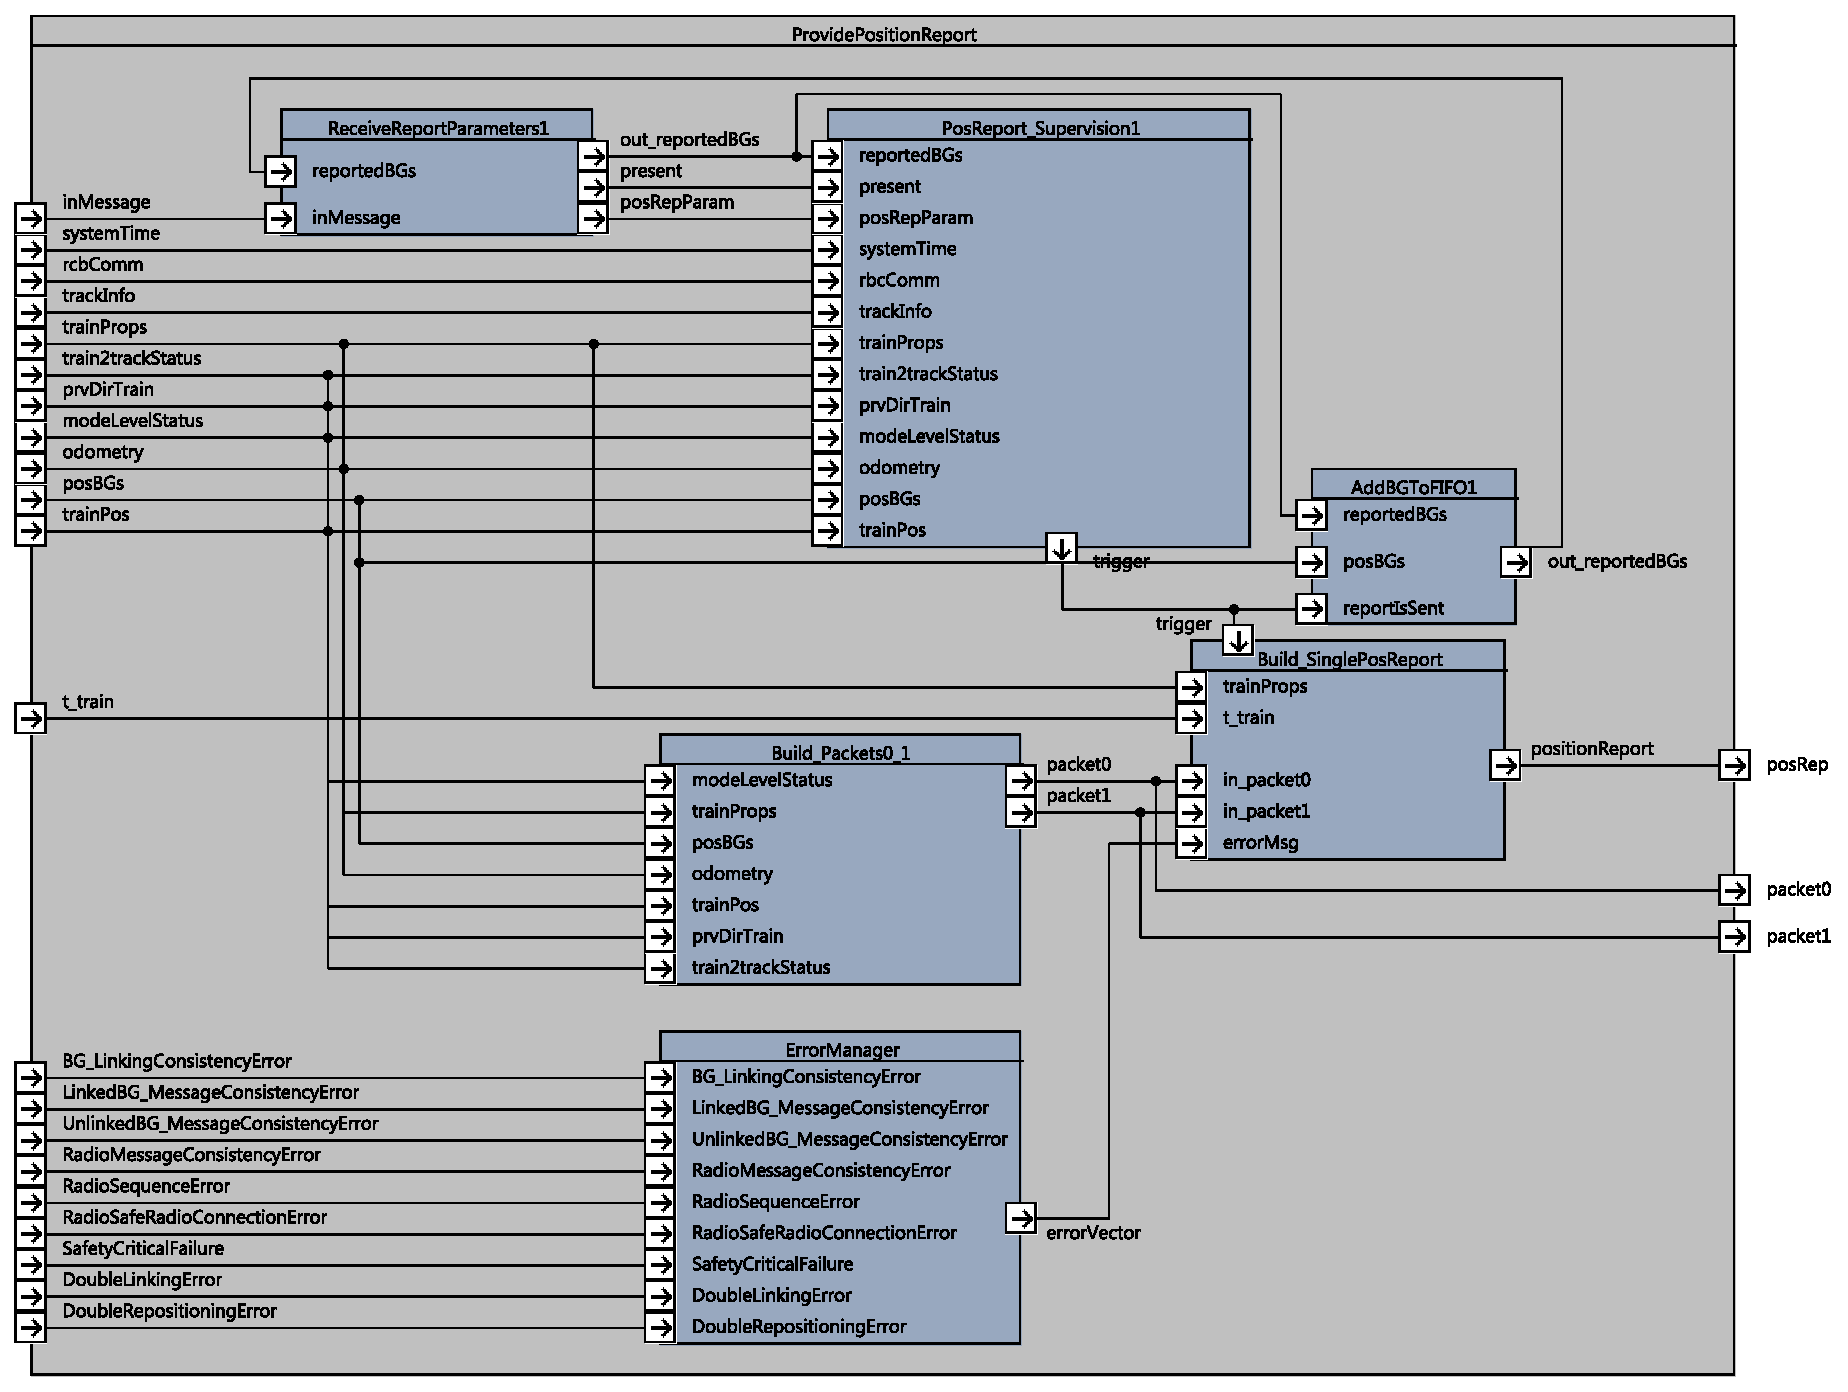
\includegraphics[width=\textwidth]{ProvidePositionReport_SysML}
\caption{Provide Position Report component SysML diagram}\label{f:provide_position_report_interface}
\end{figure}


Figure~\ref{f:provide_position_report_interface} shows the architecture of component Provide Position Report. Most of the inputs and outputs have been explained in detail in Section~\ref{s:manage_track_data_inputs} and Section~\ref{s:manage_track_data_outputs}